\subsection{Non-Premixed Combustion}

\subsubsection{What is the typical structure of a laminar diffusion flame?}

{\color{gray}\footnotesize [Claude context: check Lecture 9 (Laminar and Turbulent Flames); Maas notes Ch.13.1, 13.3, 13.4 / Warnatz Ch.13 (Nonpremixed Flames)]}

\paragraph{Answer}
Oxidizer on one side, fuel on teh other. Flame is a thin layer equilibrating trasport of both an teh products. 




\subsubsection{Why is there no such thing as a laminar flame speed of a diffusion flame?}

{\color{gray}\footnotesize [Claude context: check Lecture 9; Maas notes Ch.13 / Warnatz Ch.13 (Nonpremixed Flames)]}

\paragraph{Answer}

The laminar flame speed is not dependent on the reactants. Only on the mixing rate, this flames are limited in teh mix rate not in teh reaction rate. 




\subsubsection{Define mixture fraction. Which conditions have to be satisfied in order that mixture fraction becomes a useful variable? Explain the idea that, using mixture fraction, a non-premixed flame problem can be split into a mixing problem and a chemical problem.}

{\color{gray}\footnotesize [Claude context: check Lecture 9/10; Maas notes Ch.13 / Warnatz Ch.14 (Turbulent Non-Premixed Flames); combustion\_modeling.pdf (supplementary, verify against Warnatz/Maas)]}

\paragraph{Answer}


Mixure fraction is the fraction of mass originaly coming from the fuel side. It shoul be 1 at fuel inlet and 0 at ox inlet. it coniseders the streams are not pure fuel or ox. 

The use of mixing fraction neables te equations to be writen in terms of mixure fraction as a single difusion or trasport 8mixing) . On the line of stechometry the reaction acours

\todo{For calude: besides awsnering the questions, it shoula also contain - Define mixure fraction, how it is calcualted considering otehr species of unoure ox anf fuel. Explain how to find teh steckeometric point. Now i came across teh question of how are products dealt with in mixure fractions? awnse it. create a note that Burke-Schumann flame structure should be explaind and also the following graphs. If the folowing queston do not need it it should be explained here  }

\begin{figure}[H]
    \centering
    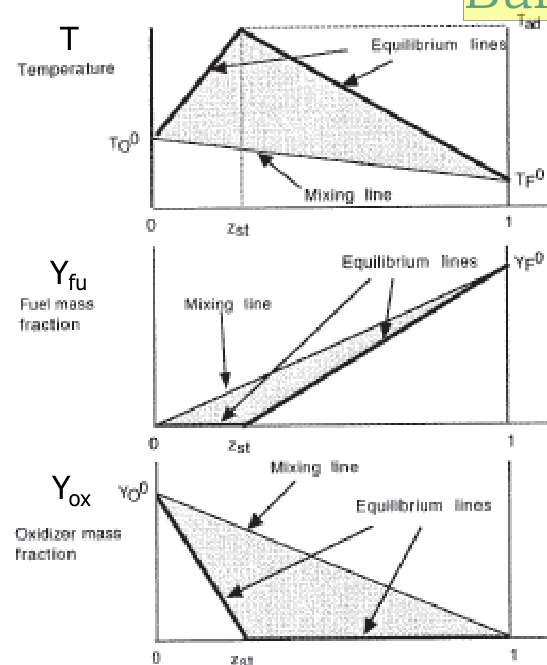
\includegraphics[width=0.5\linewidth]{ireversible.png}
    \caption{Enter Caption}
    \label{fig:placeholder}
\end{figure}

\begin{figure}[H]
    \centering
    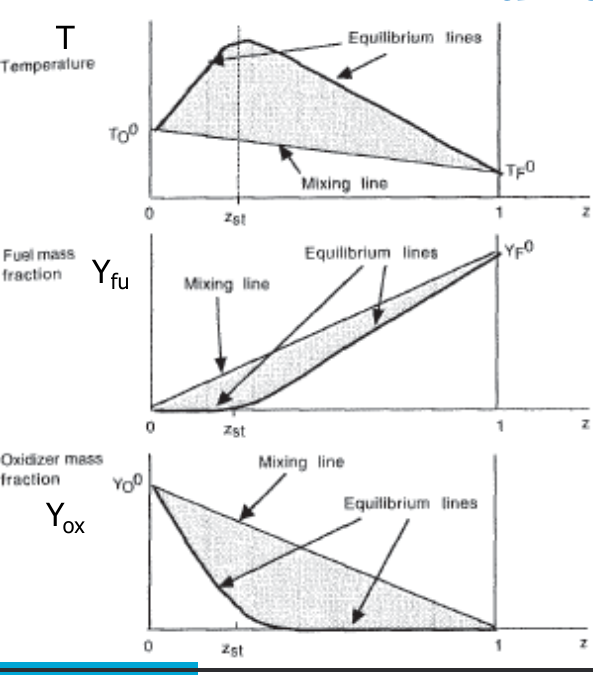
\includegraphics[width=0.5\linewidth]{reversible.png}
    \caption{Enter Caption}
    \label{fig:placeholder}
\end{figure}

\subsubsection{Define mixture fraction. In which circumstances can enthalpy be considered equivalent to mixture fraction?}

{\color{gray}\footnotesize [Claude context: check Maas notes Ch.13 / Warnatz Ch.14 (Turbulent Non-Premixed Flames); Lecture 9/10]}

\paragraph{Answer}

Enthalpy can be related to Z in wel posed bc and adiabatic systems.




\subsubsection{Explain how the influence of turbulent fluctuations of mixture fraction can be taken into account by making use of an assumed shape of its probability density function.}

{\color{gray}\footnotesize [Claude context: check Lecture 10; Warnatz Ch.14 (Turbulent Non-Premixed Flames, presumed PDF approach); combustion\_modeling.pdf (supplementary, verify against Warnatz)]}


\paragraph{Answer} problem with averaging quantities has been previusly explained, as well as pdf and montecarlo methods. 

\todo{For calude: is this the same question? y is this here, any ways.. make any relevant diferneces or reexplain hw the previus }






\subsubsection{Explain why one is interested in calculating the variance of mixture fraction. How does the scalar dissipation rate influence the variance of mixture fraction?}

{\color{gray}\footnotesize [Claude context: check Lecture 10; Warnatz Ch.14 (mixture fraction variance, scalar dissipation rate); combustion\_modeling.pdf (supplementary, verify against Warnatz)]}

\paragraph{Answer}

Mixure fration variation is used to find the point where flame is. Ak point of stochiometric conditions. 

When the change of coordinates is introduced, to Z and its notmal coterpats, equations are rewritan and flmelet equations obtained. These equations need te concetration of species as a function of Z




\subsubsection{Explain the steady laminar flamelet model of turbulent non-premixed combustion.}

{\color{gray}\footnotesize [Claude context: check Lecture 10; Warnatz Ch.14 (flamelet model for non-premixed combustion); combustion\_modeling.pdf (supplementary, verify against Warnatz)]}

\paragraph{Answer}
Flamelet assumes mixing does ot hapen in the flame. that the cheical time scales are much faster than mixing time scales. 
... lecture 9 





